\documentclass[12pt]{cornelltfpxsop}
\title{Dee construction: Gluing  parts into Dee mechanical structure}
\date{\today}
\author{M.Acero, T.Babenko, A.Daoud, J.Monroy, D.Velázquez}
\approved{Jose Monroy}
\usepackage{graphicx}
\usepackage{float}
\usepackage{subcaption}
\usepackage{paracol}
\setlength{\columnseprule}{0.4pt}

\sopid{DC}
\sopversion{V5}
\sopabstract{Describes the procedures to glue co-cured Carbon fiber-foam halves housing PEEK inserts, and titanium flower pattern evaporator, using the robotic gantry. The procedure takes place in the clean room. This is a two-person procedure.}



\begin{document}

\maketitle
%------------------------------------------------------------------
\section{Scope}
This process describes the assembly of the D-shaped mechanical structure (''Dee'') stage for the TFPX cartridge integration process.

%------------------------------------------------------------------
\section{Purpose}
The ``Dee'' is the mechanical structure that supports the silicon modules. It also provides cooling and support for power cables and e-links.    

%------------------------------------------------------------------
\section{Definitions}
\begin{center}
\begin{figure}[h!]
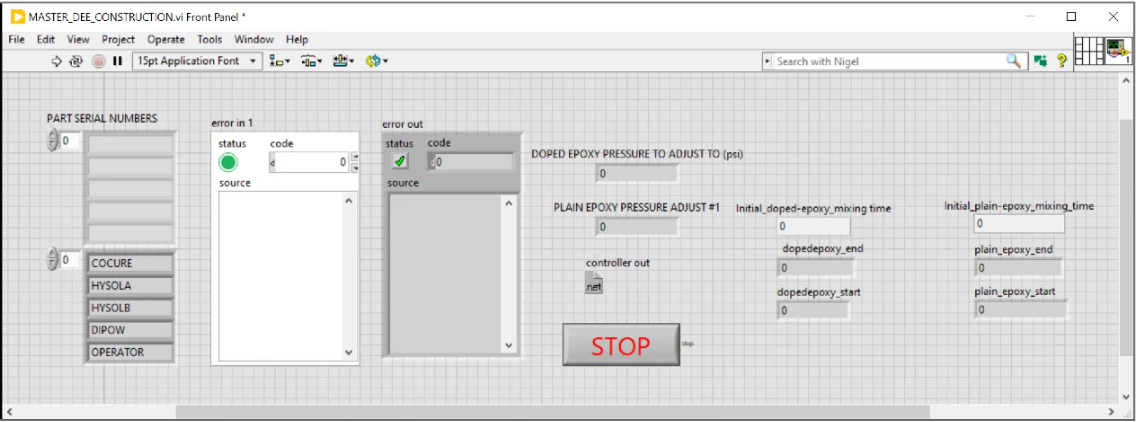
\includegraphics[width=\textwidth]{img2/FrontPanel.png}
\caption{Front Panel of MASTER\_DEE\_CONSTRUCTION.vi}
\label{front_panel}
\end{figure}
\end{center}

\begin{itemize}
    \item Motion Composer: is a program that runs GCODE. GCODE is a set of instructions for the Gantry to move along. Think of a GCODE path like the path a paintbrush needs to be moved along to make a painting.
    %\item For all the GCODE programs, there is a delay of about 5 seconds to allow user to position near the NPaq switch just in case.
    \item Flower Pattern: The cooling tube or evaporator has a flower shape which we call here the flower pattern. The Gantry needs to deposit epoxy while it is moving along the flower pattern path in the Dee. For this, we have a GCODE script/program run by Motion composer.
    \item Carbon fiber-foam co-cure (CFF): The Dee structure is formed by two skins of carbon fiber and two bodies of carbon foam. One carbon fiber skin and carbon foam are co-cured in one entity, so that the Dee is composed of 2 halves of CFF (CFF\_A and CFF\_B). In between the two CFF, inserts and evaporator are sandwiched.    
    \item Insert Filling: Dee has some PEEK inserts that will serve as clamping points for structures/objects on it. The Gantry moves to the location of the insert holes and deposit epoxy while STOPPED at that position. 
    \item Front panel: It is the window through which the user interact with the LabVIEW control program. It shows statistical information, status of the vacuum system, tools and elements in use and other relevant information (see figure \ref{front_panel})
\end{itemize}

%------------------------------------------------------------------
%\section{Responsibilities}

%------------------------------------------------------------------
\section{Equipment}
\begin{figure}[H]
    \centering
    \begin{subfigure}[b]{0.45\textwidth}
        \centering
        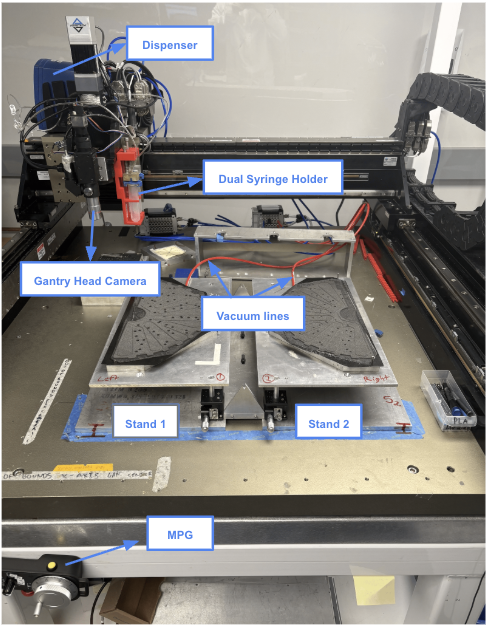
\includegraphics[width=\textwidth]{img2/Gantrysetup.png}
        \caption{Gantry setup. Labels indicate the main parts of the setup.}
        \label{fig:gantry_setup}
    \end{subfigure}
    \hfill
    \begin{subfigure}[b]{0.45\textwidth}
        \centering
        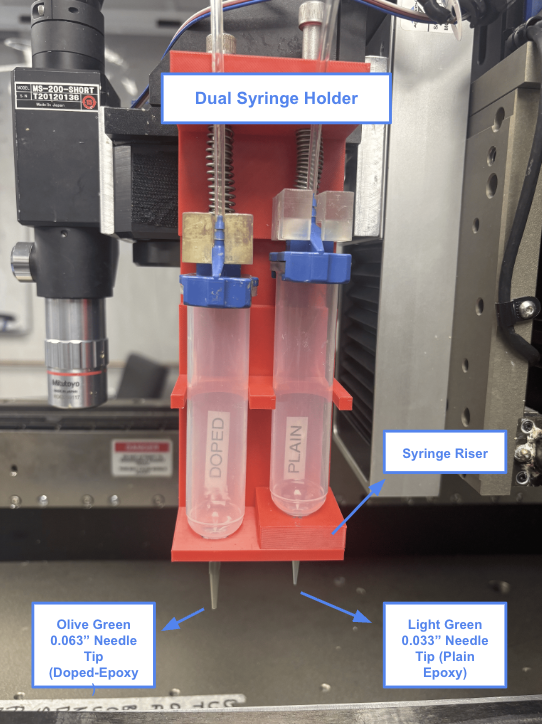
\includegraphics[width=\textwidth]{img2/syringe_holder2.png}
        \caption{Dual Syringe Holder. Labels indicate key attributes of the holder.}
        \label{fig:second_image}
    \end{subfigure}
    \caption{Primary Equipment and Setup for Dee Construction.}
    \label{fig:main_setup}
\end{figure}

\begin{enumerate}

\item Gantry (check that everything (labeled in the figure  \ref{fig:gantry_setup}) is installed and working properly. 
    \begin{itemize}[itemsep=0.5pt,parsep=0pt,topsep=4pt]
        \item Dual syringe holder and U-shaped riser block (Figure \ref{fig:second_image})
        \item Stands with alignment screws
        \item Pressurized air dispenser -- Ultimus II
        \item Dispenser foot pedal
        \item Two blue pressure-cap and hose assemblies for the gantry syringes
        \item MPG controller
        \item Compressed air lines with splitter
        \item Vacuum manifold and lines
    \end{itemize}
\newpage
\item Parts and tools
\begin{figure}[H]
    \centering
    \setlength{\tabcolsep}{6pt}
    \begin{tabular}{cc}
        \includegraphics[width=0.44\linewidth,height=1.5in,keepaspectratio]{img2/DEEs.png} &
        \includegraphics[width=0.44\linewidth,height=1.5in,keepaspectratio]{img/PartsTools_2.png} \\[4pt]
        \includegraphics[width=0.44\linewidth,height=1.5in,keepaspectratio]{img2/Centrifuge.png} &
        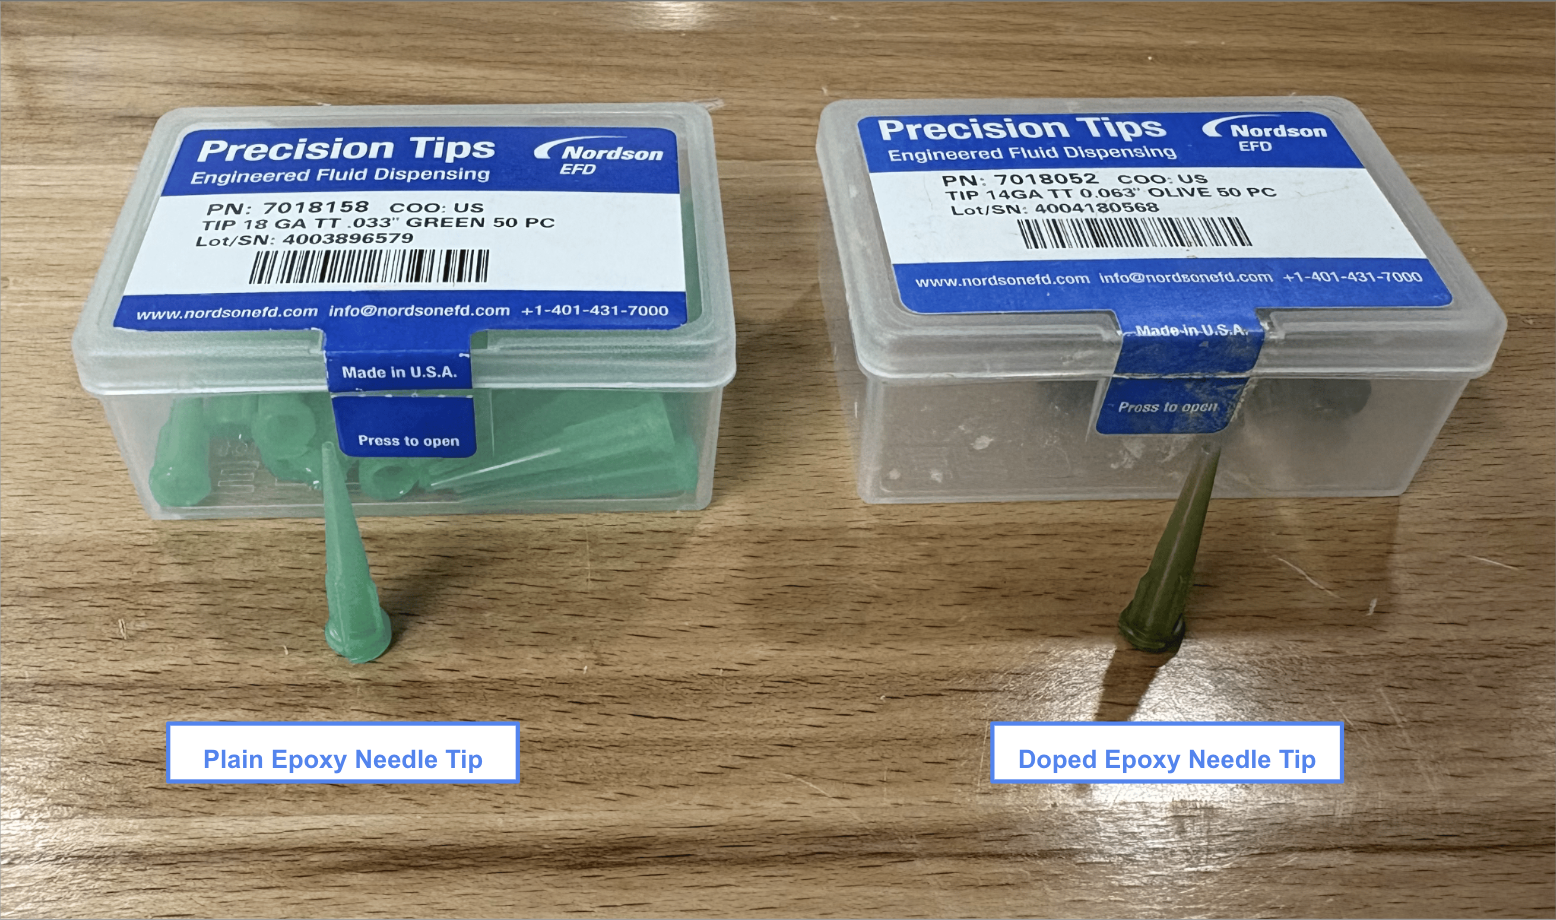
\includegraphics[width=0.44\linewidth,height=1.5in,keepaspectratio]{img2/needle_tips.png}
    \end{tabular}
    \captionsetup{font=small,skip=6pt}
    \caption{Parts and tools used in the DEE manufacturing process. Materials listed for epoxy preparation should be located on the table inside room PSB 375 where the epoxy mixing will be performed; the rest of materials must be located on the table in front of the gantry except for evaporator, inserts and tweezers which should be located on the table left to the gantry.}
\label{Parts ands tools}
\end{figure}
    \begin{itemize}[itemsep=0.5pt,parsep=0pt,topsep=4pt]
        \item Side A Half-Dee CFF\_A 
        \item Side B Half-Dee CFF\_B
        \item PEEK Periphery
        \item EA9396 Epoxy  parts A and B. 
        \item Flower-Pattern Shape Titanium $CO_2$ tube/evaporator
        \item 0.063" Olive green Nordson fluid dispensing tip
        \item 0.033" Light green Nordson fluid dispensing tip
        \item Box with PEEK inserts (56 will be used)
        \item Tweezers
        \item Two bottom jig plates (with vacuum lines)
        \item One top jig plate
        \item Both 3D-printed pressing tools for seating the evaporator and inserts
        \item Flower-pattern cover piece for spreading epoxy on Side B
        \item Plastic scraper for spreading doped epoxy over Side B
        \item Small scraping tool/spatula for clearing epoxy from the filling holes
        \item Neodymium magnets for securing CFF Half-Dee to Jig plate
        \item Small soft paint brush
        \item Curing oven
        \item Painter's Tape
    \end{itemize}
\newpage
\item Epoxy preparation \textbf{(Performed in PSB 375)}
    \begin{itemize}[itemsep=0.5pt,parsep=0pt,topsep=4pt]
        \item Two preweighed bags of 12--20 micron diamond powder, 29.4~g each
        \item EA9396 Epoxy Part A
        \item EA9396 Epoxy Part B
        \item Three separate manual syringes preloaded with Part B: two containing 2.9~g each and one containing 4.6~g
        \item 2 Popsicle Sticks
        \item Two large gantry syringes, two pistons, and two blue stopper caps
        \item One small handheld syringe with plunger for manual plain-epoxy filling on Side A, with a dispensing tip if used
        \item Thin spatula for mixing plain epoxy inside the large gantry syringe
        \item Digital Scale
        \item Centrifuge
        \item Designated counterweight matched to the loaded flower-pattern doped-epoxy syringe (identifying label or target mass to be confirmed)
        \item Paper Towels
        \item Isopropyl Alcohol
        \item Two rubber mixing beakers: one for flower-pattern doped epoxy and one for spreading doped epoxy
        \item Nitrile Gloves
        \item Face Mask
        \item Box Fan
        \item Painter's Tape
    \end{itemize}
\end{enumerate}
\clearpage
%------------------------------------------------------------------
\begin{figure}[h]
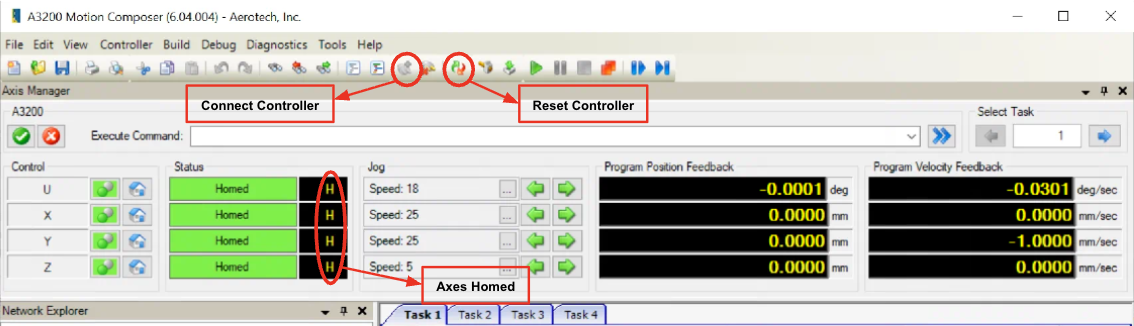
\includegraphics[width=1\textwidth,angle = 0]{img2/motioncomposer.png}
\caption{Motion Composer software used to operate gantry, MPG, and run G-CODE scripts for deposition.}
\label{motion_composer}
\end{figure}

\section{Procedure}
\subsubsection*{Person 1:}
\begin{enumerate}
    \item Check that the NPAQ, power supplies, dispenser, and vacuum pumps are turned on. Turn on any if necessary.
    \item Check that the compressed air lines are open.
    \item Open the LabVIEW control software:\\
    \verb|C:\Users\co2_clt\Documents\MASTER_DEE_Construction|\\
    \verb|\MASTER_DEE_CONSTRUCTION_S26.vi|\\
    Ensure that it opens in LabVIEW 2025.
    \item Open Motion Composer.
    \item Check that no other Gscript or LabVIEW programs are running that could interfere with the deposition.
    \item Make sure the gantry is connected in Motion Composer, as shown in Figure~\ref{motion_composer}. The elongated circle should show H's (Home), not VH's (Virtual Home). If VH is shown, the NPAQ is likely turned off.
    \item Ensure that the MPG program is running in Motion Composer and check that the MPG is working properly. MPGSample should be running and dwelling on \textit{Program Pause}.
    \item Test the dispenser and vacuum using the test programs in the same folder:
    \begin{enumerate}
        \item \textbf{Dispenser\_Shot.vi} tests the dispenser.
        \item \textbf{manifold.vi} tests the vacuum.
    \end{enumerate}
    \item Identify the parts. Handle them with gloves and a face mask. Check that the parts are in good condition.
    \item Assign a new unique Dee number (\texttt{D\_xxx}).
    \item Run \verb|MASTER_DEE_CONSTRUCTION_S26.vi| and provide the required information:
    \begin{enumerate}
        \item Part numbers.
        \item Dee identification.
        \item Other required information.
    \end{enumerate}
    \item Mount the bottom jig plate onto Stand 1 and align it using the alignment screws (Figure~\ref{JigAlignment}).
\begin{figure}[H]
        \centering
        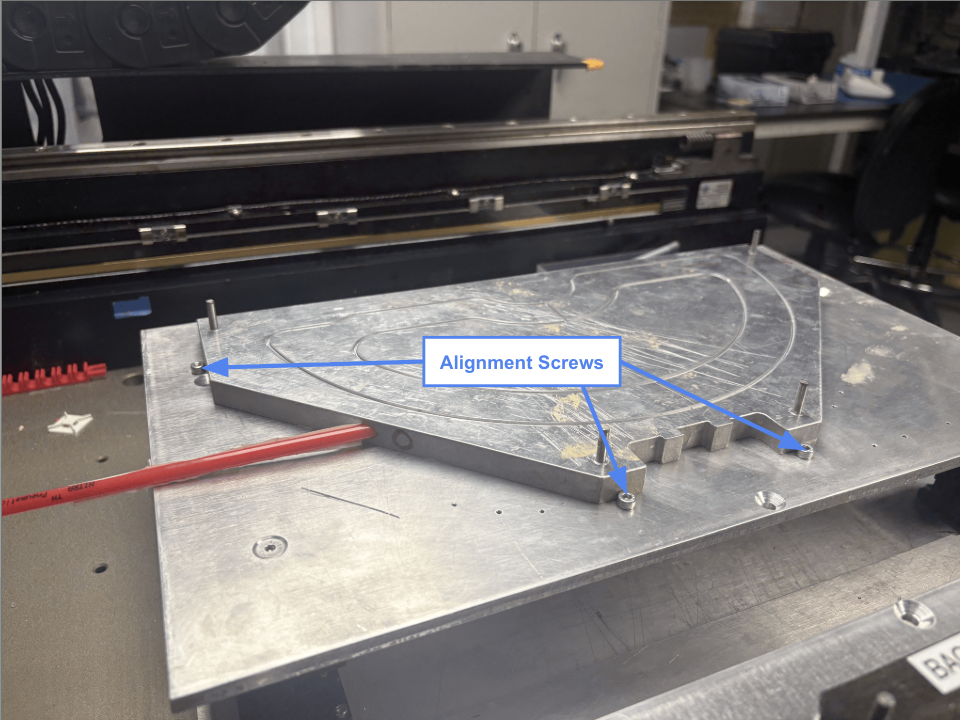
\includegraphics[width=.4\linewidth]{img2/jig_alignment2.png}
        \caption{Jig alignment}
        \label{JigAlignment}
    \end{figure}
    \item Connect the labeled vacuum line to the corresponding bottom jig.
    \item Mount CFF\_A onto the bottom jig plate on Stand 1 using the jig poles and holes in CFF\_A.
    \item Mount CFF\_B onto its bottom jig plate and place it on Person 2's worktable. Person 2 will spread doped epoxy on Side B while Side A's depositions are running, then return Side B to Stand 2.
    \item Use the neodymium magnets to secure the CFF halves onto their jig plates. Place them around the edges of the CFF halves. The magnets should lock into the correct positions. Keep each cocure half attached to its bottom jig plate during transfers between the worktable and gantry.
\begin{figure}[H]
    \centering
    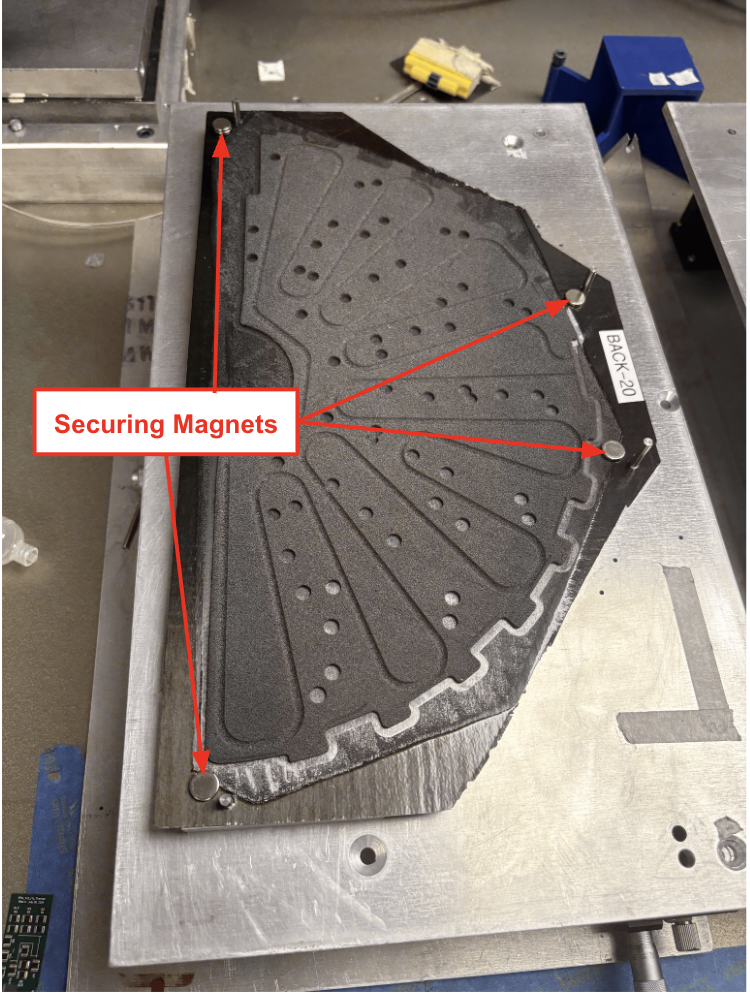
\includegraphics[width=0.4\linewidth]{img2/Magnets2.png}
    \caption{Neodymium magnets used to secure CFF halves onto the jig plates.}
    \label{magnets}
\end{figure}
    \item After Person 2 comes into the clean room with both gantry syringes, the spreading beaker, and the handheld plain-epoxy syringe, the control program will have moved the gantry to the front of the table for syringe installation. Receive both gantry syringes and screw the blue pressure cap and hose assembly onto them. Person 2 keeps the spreading beaker and handheld syringe.
    \item Obtain the two recorded start times from Person 2: when Part B was added to the flower-pattern doped epoxy and when it was added to the plain epoxy. When prompted, enter the elapsed age of each epoxy in minutes. The program adds the time elapsed between later steps to these initial ages to determine the dispensing pressure.
    \item Unscrew the blue stopper caps at the bottom of both syringes. Install the \textit{olive green 0.063-inch tip} onto the doped-epoxy syringe and the \textit{light green 0.033-inch tip} onto the plain-epoxy syringe. Load both syringes into their designated positions on the dual syringe holder.
    \item Use the dispenser pressure foot pedal and pressure splitters to fill each syringe tip with epoxy so that no air bubbles remain in the tips. Use a pressure $\leq 5.5$~PSI for plain epoxy and $\leq 40.0$~PSI for doped epoxy. Wipe any epoxy from the tips. Select ``Okay'' when both syringes are installed and the tips are filled.
    \item Initially, place the U-shaped riser block under the unused plain-epoxy syringe to keep it elevated (Figure~\ref{fig:second_image}). The doped-epoxy syringe should be in its dispensing position, with the compressed air splitter open to it.
    \item The program will send the gantry home and prompt you before flower-pattern deposition begins. Perform the final checks listed on the front panel, then select ``FPAT A''. The gantry will move to the start of Side A's flower pattern.
    \item Check that the olive needle tip is directly over the starting point of the flower-pattern line, as shown in Figure~\ref{needleref}. Adjust it using the MPG if needed.
\begin{figure}[H]
            \centering
            \includegraphics[width=0.45\linewidth]{img2/FPATstart1.png}
            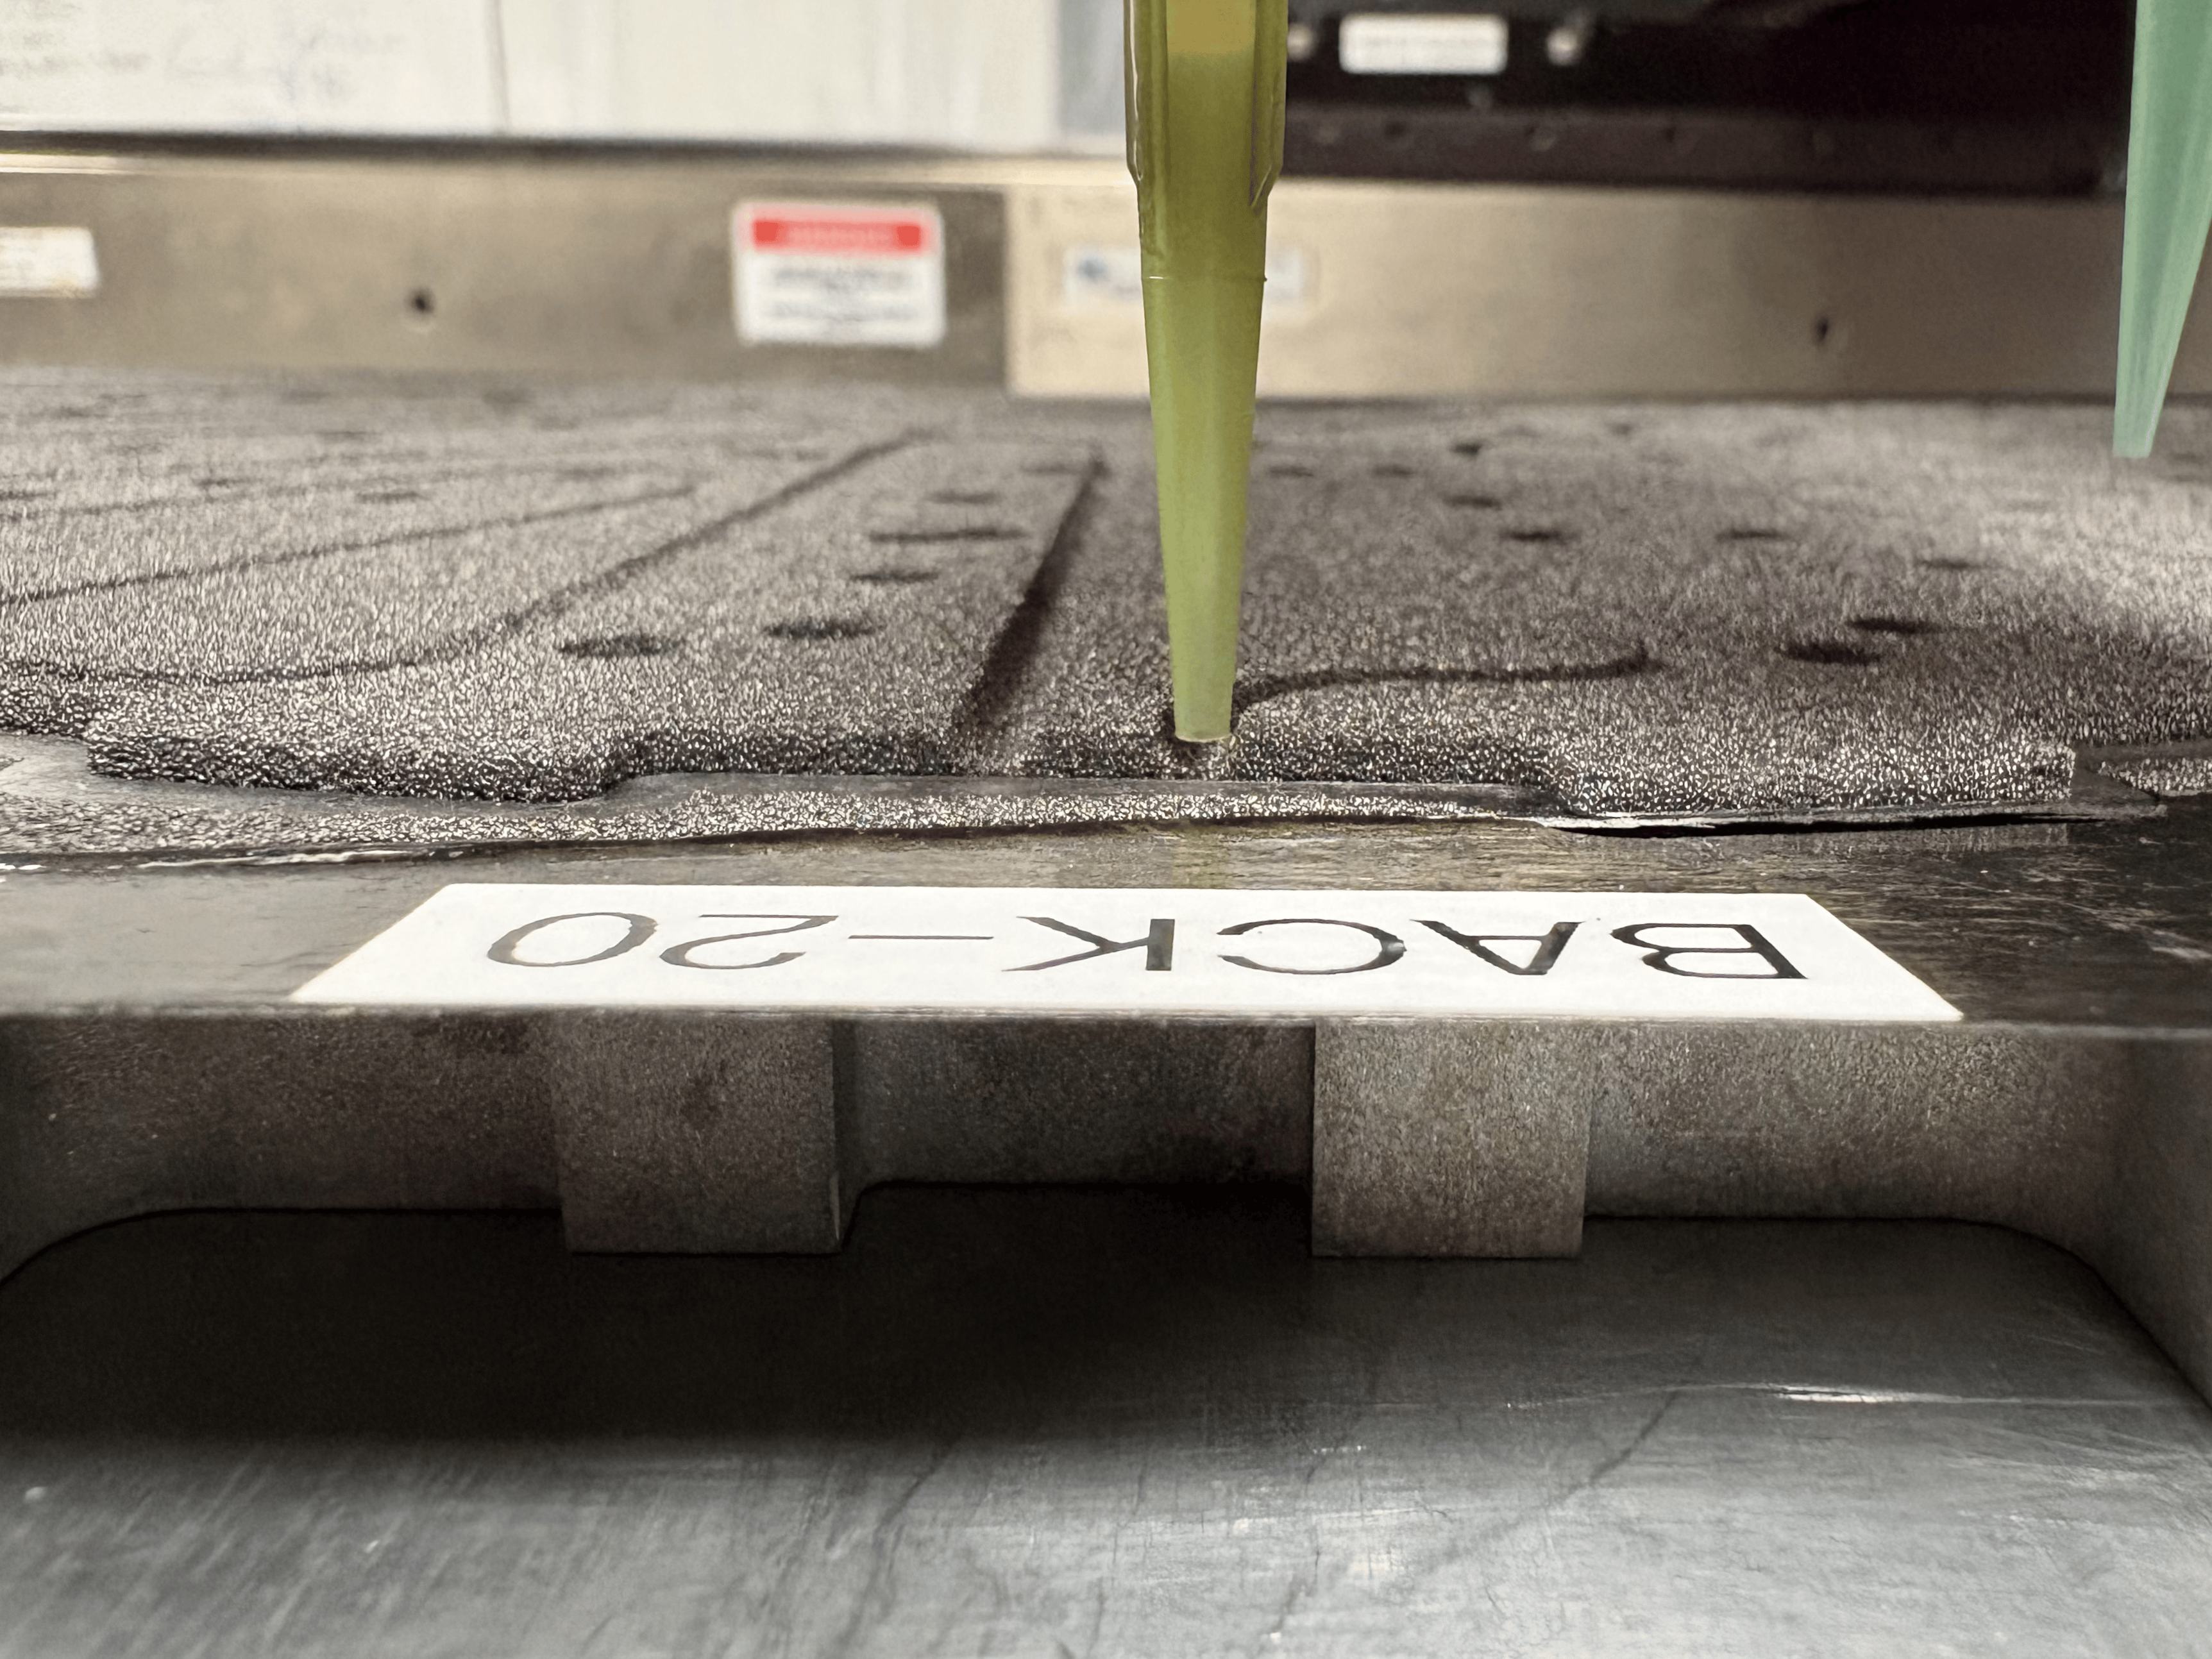
\includegraphics[width=0.45\linewidth]{img2/FPATstart2.png}
            \caption{Needle starting position}
            \label{needleref}
        \end{figure}
    \item \textbf{[Flower Pattern Side A]} Adjust the pressure to the value provided by the program. Begin doped-epoxy deposition by selecting ``OK'' on the pressure-adjustment prompt. Check for consistent epoxy flow and adjust the pressure if needed during deposition.
    \item Immediately after flower-pattern deposition ends, inspect the deposition. When prompted, select ``YES'' if another flower-pattern pass is needed on top of the existing deposition. Keep the doped syringe selected and follow the repeat prompts. Select ``NO'' when sufficient epoxy has been deposited.
    \item \textbf{[Periphery Side A]} After accepting the flower-pattern deposition, switch the compressed airflow to the plain-epoxy syringe. Move the U-shaped riser block from beneath the plain syringe to beneath the doped syringe, leaving the plain syringe in its dispensing position. Adjust the pressure according to the prompt. Check that the light green tip is aligned with the starting position for Side A's periphery, adjust with the MPG if needed, and select ``OK'' to begin. There is no repeat option for periphery deposition.
    \item After periphery deposition ends, the gantry head will move out of the way of CFF\_A. Person 2 disconnects its vacuum line and moves CFF\_A together with its bottom jig plate to the worktable. Person 2 then installs the periphery and evaporator, followed by manually filling the holes and installing the inserts. There is no automated filling deposition on Side A.
    \item Before starting Side B, confirm that Person 2 has finished spreading its doped epoxy, cleared the filling holes, removed the flower-pattern cover, and returned CFF\_B with its bottom jig plate to Stand 2. Person 2 reconnects the labeled vacuum line. Confirm that Side B is secured and ready for deposition.
    \item Switch the compressed airflow back to the doped-epoxy syringe. Move the U-shaped riser block from beneath the doped syringe to beneath the plain syringe, leaving the doped syringe in its dispensing position.
    \item Check that the olive needle tip is at the starting point for Side B's flower pattern. Adjust its position with the MPG if needed and adjust the pressure according to the front-panel prompt.
    \item \textbf{[Flower Pattern Side B]} Begin epoxy deposition by selecting ``OK'' on the front panel. Check for consistent epoxy flow.
    \item Immediately after flower-pattern deposition ends, inspect the deposition. When prompted, select ``YES'' if another flower-pattern pass is needed on top of the existing deposition. Keep the doped syringe selected and follow the repeat prompts. Select ``NO'' when sufficient epoxy has been deposited.
    \item After accepting the flower-pattern deposition, the gantry will move to the starting position for Side B's periphery. Switch the compressed airflow to the plain-epoxy syringe. Move the U-shaped riser block from beneath the plain syringe to beneath the doped syringe. Check the light green tip position and adjust it if needed. Adjust the pressure according to the front-panel prompt.
    \item \textbf{[Periphery Side B]} Select ``OK'' to begin depositing plain epoxy around the edges of CFF\_B. There is no repeat option for periphery deposition.
    \item After periphery deposition ends, the gantry will move to the starting position for Side B's filling-hole deposition. Keep the plain syringe selected and the doped syringe elevated. Adjust the needle position with the MPG if needed and adjust the pressure according to the front-panel prompt.
    \item \textbf{[Filling Side B]} Select ``OK'' to begin filling deposition.
    \item Immediately after filling deposition ends, inspect the filling holes. When prompted, select ``YES'' if another filling pass is needed. Keep the plain syringe selected and follow the repeat prompts, adjusting the pressure if needed. Select ``NO'' when sufficient epoxy has been deposited.
    \item After Side B's depositions are complete, have Person 2 disconnect its vacuum line. Remove CFF\_B together with its bottom jig plate from the gantry table and bring it to Person 2's worktable.
    \item Confirm that Person 2 has completed Side A's assembly: the periphery, evaporator, and all manually filled inserts must be installed before stacking. If assembly is not complete, wait until Person 2 confirms it is ready.
    \item Flip CFF\_B so that the carbon foam faces down. \textbf{The handling of Side B's bottom jig plate during this step remains to be confirmed.}
    \item Use the poles on the bottom jig to stack CFF\_B on top of CFF\_A.
    \item Stack the top jig plate on top of CFF\_B. Make sure all pieces fit into place and the holes are aligned.
    \item Take the full stack into the oven. Turn on the oven and bake for 2 hours at $50\,^{\circ}\mathrm{C}$, followed by 4 hours of cooling. Follow the instructions fixed to the oven door (Figure~\ref{oven}).
    \item Clean up the working space.
\begin{figure}[h]
            \centering
            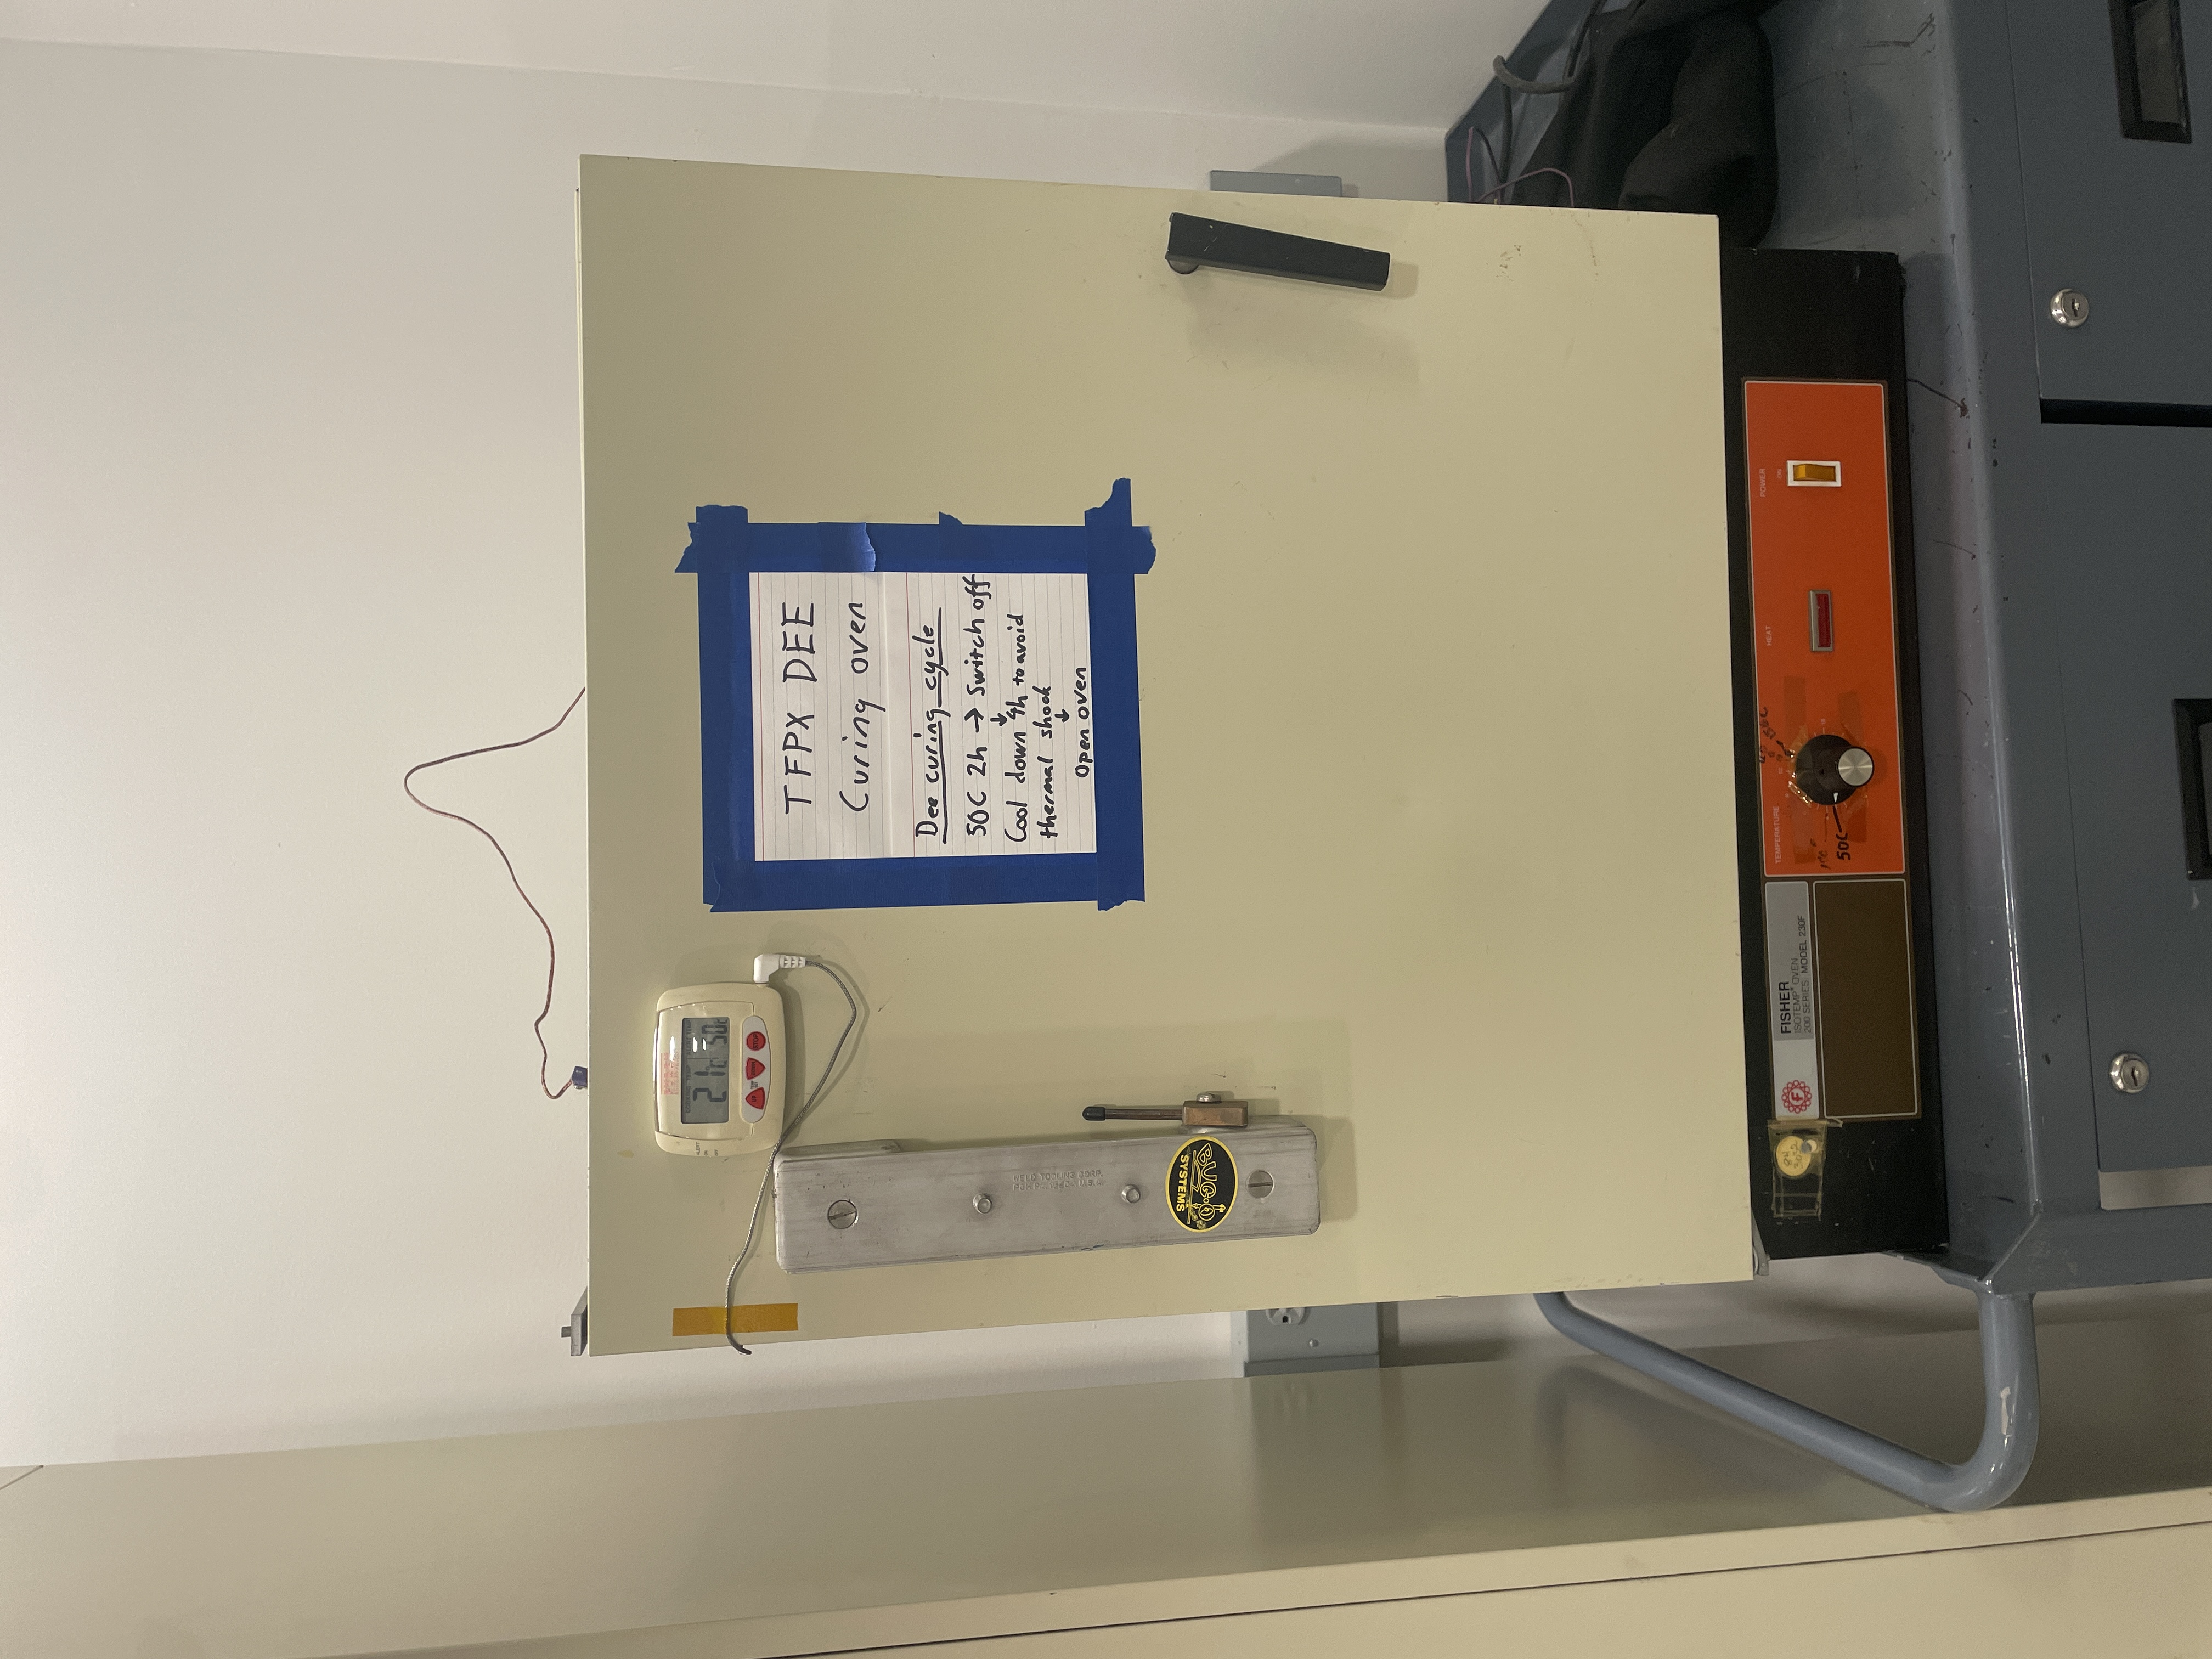
\includegraphics[width=0.4\linewidth, angle=-90]{img/oven.JPG}
            \caption{Oven for curing Dee after assembly}
            \label{oven}
        \end{figure}
\end{enumerate}
\newpage
\subsubsection*{Person 2:}
\begin{enumerate}
    \item Prepare the mixing area, scale, tools, and centrifuge. Ventilate the room with the fan. Put on a face mask and gloves, cover the table with paper towels, and tape them in place. Set the scale to grams.

    \item Label two beakers:
    \begin{itemize}
        \item \textbf{Flower pattern:} doped epoxy for the gantry syringe.
        \item \textbf{Spreading:} doped epoxy for spreading on Side B (CFF\_B).
    \end{itemize}

    \item Prepare each beaker separately. Zero the scale with the empty beaker in place, then weigh \textbf{9.7~g of EA9396 Part A} into it.

    \item Empty one prepared \textbf{29.4~g bag of diamond powder} into each beaker. Mix the diamond thoroughly into Part A. Do not add Part B yet.

    \item Fit the stopper cap to the plain-epoxy gantry syringe. Zero the scale with the capped syringe in place, then weigh \textbf{15.4~g of Part A directly into the syringe}. Leave it there until ready to add Part B.

    \item Have the premeasured Part B portions ready in separate manual syringes:
    \begin{itemize}
        \item \textbf{2.9~g} for the flower-pattern beaker.
        \item \textbf{2.9~g} for the spreading beaker.
        \item \textbf{4.6~g} for the plain-epoxy syringe.
    \end{itemize}
    Each doped batch will total \textbf{42.0~g}. The plain batch will total \textbf{20.0~g}. The Part A and Part B amounts follow the \textbf{10:3 ratio by mass}, rounded to 0.1~g. Use these batch quantities for this procedure.
    \begin{figure}[H]
        \centering
        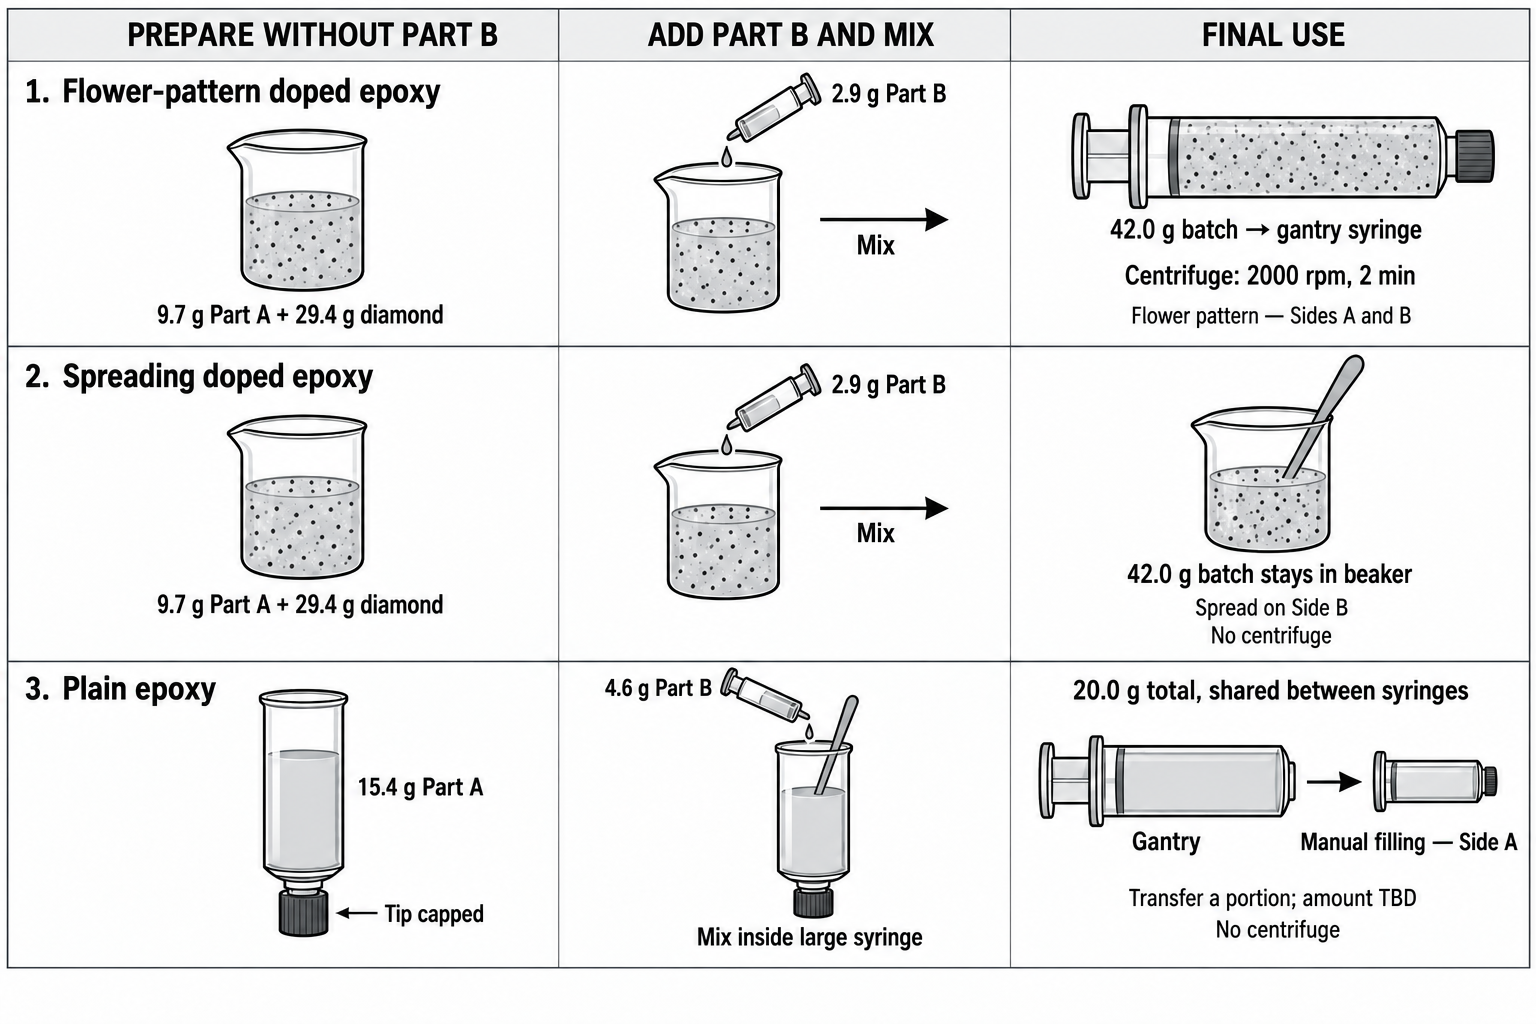
\includegraphics[width=\linewidth]{img/epoxy_preparation.png}
        \caption{Epoxy preparation and intended use of the three batches.}
        \label{fig:epoxy_preparation}
    \end{figure}

    \item Add \textbf{2.9~g of Part B} to the flower-pattern beaker and begin mixing immediately. Record the clock time, to the nearest minute, when Part B is added. This is the \textbf{flower-pattern doped-epoxy start time}.

    \item Mix thoroughly, then transfer the flower-pattern epoxy into its gantry syringe. Fit the stopper cap before filling the syringe, and install the piston before centrifuging.

    \item Place the loaded flower-pattern syringe in the centrifuge opposite its designated matching counterweight. Centrifuge at \textbf{2000~rpm for 2~minutes}. \textbf{Only the flower-pattern doped-epoxy syringe is centrifuged.}

    \item Next, add \textbf{2.9~g of Part B} to the spreading beaker and mix thoroughly. Keep this epoxy in the beaker. No start time needs to be recorded for this batch.

    \item Add \textbf{4.6~g of Part B} to the plain-epoxy gantry syringe containing \textbf{15.4~g of Part A}. Immediately mix thoroughly inside the syringe using a thin spatula. Record the clock time, to the nearest minute, when Part B is added. This is the \textbf{plain-epoxy start time}.

    \item After mixing, manually extrude a portion of the plain epoxy from the large syringe into the smaller handheld syringe. Keep the remainder in the large syringe for the gantry depositions. \textbf{Amount to transfer: to be determined.} The 20.0~g batch is shared between both syringes. Do not centrifuge either plain-epoxy syringe.

    \item Follow the clean-room dressing procedure before entry. Bring the following into the clean room:
    \begin{itemize}
        \item Flower-pattern doped-epoxy gantry syringe.
        \item Plain-epoxy gantry syringe.
        \item Beaker of doped epoxy for spreading.
        \item Small handheld syringe of plain epoxy.
    \end{itemize}

    \item Give both gantry syringes to Person 1. Provide the recorded start times for the flower-pattern doped epoxy and the plain epoxy.

    \item Person 1 enters each epoxy's elapsed age, in minutes, into LabVIEW. LabVIEW uses these initial ages and adds the time elapsed between later steps to calculate the dispensing pressure. The plain epoxy in the handheld syringe has the same start time as the plain epoxy in the gantry syringe.

    \item While Person 1 runs the \textbf{flower-pattern and periphery depositions on Side A (CFF\_A)}, prepare Side B on the worktable. Place the flower-pattern cover over Side B's flower-pattern grooves. Have the inserts, periphery pieces, evaporator, and pressing tools ready on the worktable.

    \item Use the doped epoxy from the \textbf{spreading beaker} to spread epoxy over the carbon-foam surface of Side B.

    \item Use the small spatula to remove any doped epoxy from Side B's filling holes. Remove the flower-pattern cover after the holes are cleared.

    \item Return the prepared Side B to its jig on Stand 2 of the gantry table before Person 1 begins Side B's depositions.

    \item Receive Side A from Person 1 on the worktable after its flower-pattern and periphery depositions are complete. \textbf{There is no automated filling-hole deposition on Side A.}

    \item Install the periphery pieces on Side A, then install the evaporator in its groove. Use the designated pressing tools (Figure~\ref{fig:pressing}) as needed to seat the parts without damaging the carbon foam.
\begin{figure}[H]
    \centering
    \includegraphics[width=0.4\linewidth]{img2/pressingpieces.png}
    \caption{Pieces used for pressing inserts and evaporator into Dee}
    \label{fig:pressing}
\end{figure}

    \item Use the small handheld syringe to fill Side A's insert holes \textbf{one at a time}:
    \begin{itemize}
        \item Deposit a drop of plain epoxy into one hole.
        \item Place an insert into that hole.
        \item Seat the insert with the designated pressing tool.
        \item Repeat for the next hole until all inserts are installed.
    \end{itemize}
\begin{figure}[H]
    \centering
    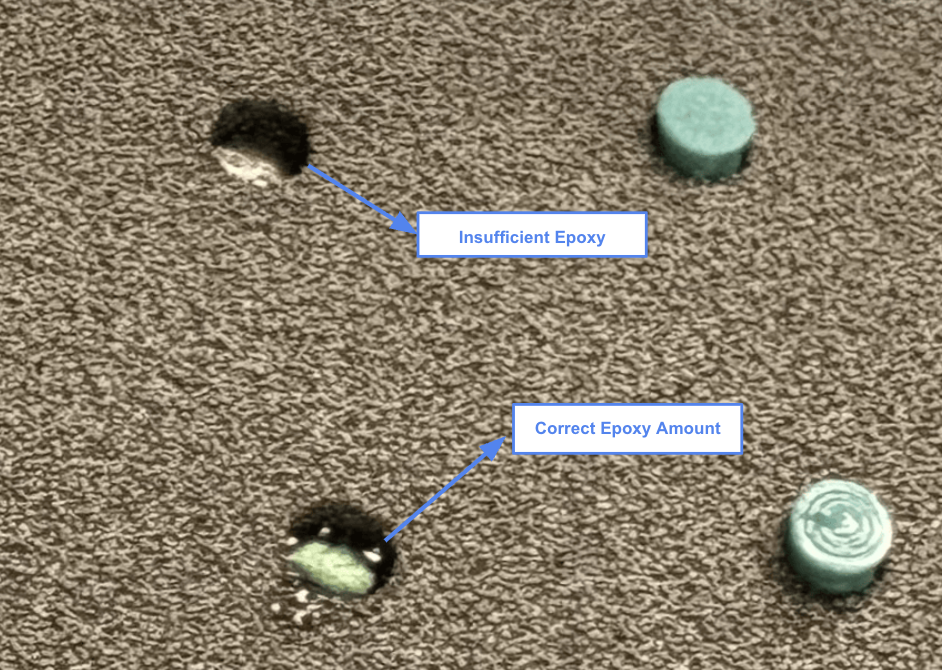
\includegraphics[width=0.6\linewidth]{img2/Epoxy_fillings.png}
    \caption{Plain epoxy filling hole examples}
    \label{epoxyref}
\end{figure}

    \item Have the top jig plate ready for final assembly when Person 1 brings over Side B.

    \item After assembly, clean the work area, beakers, and tools. Use isopropyl alcohol to clean the beakers and wipes to clean the surfaces and tools.
\end{enumerate}
%------------------------------------------------------------------
\section{Documentation}

Any special observations, e.g. damage to parts not already recorded during visual inspection, deviations from normal procedures, should be added to the report in the last step of the routine in the comments pop-up window 

The following information is recorded in the report generated by the gluing software:
\begin{itemize}
    \item Date, time (start--end) and operator name
    \item Time stamps at the start of each deposition stage
    \item Id of parts used:
	\begin{itemize}
	    \item Carbon fiber-foam: S/N
	    \item Dee ID
	    \item Epoxy information
	\end{itemize}
    \item observations/comments
\end{itemize}

Find the report at \\ \verb| C:\Users\co2_ctl\Documents\MASTER_DEE_Construction\LOGS\|.\\ Write an ELog entry and upload the report to it and to the appropriate DataBase.  

\end{document}

